% Options for packages loaded elsewhere
\PassOptionsToPackage{unicode}{hyperref}
\PassOptionsToPackage{hyphens}{url}
%
\documentclass[
  12pt,
]{article}
\usepackage{amsmath,amssymb}
\usepackage{lmodern}
\usepackage{iftex}
\ifPDFTeX
  \usepackage[T1]{fontenc}
  \usepackage[utf8]{inputenc}
  \usepackage{textcomp} % provide euro and other symbols
\else % if luatex or xetex
  \usepackage{unicode-math}
  \defaultfontfeatures{Scale=MatchLowercase}
  \defaultfontfeatures[\rmfamily]{Ligatures=TeX,Scale=1}
\fi
% Use upquote if available, for straight quotes in verbatim environments
\IfFileExists{upquote.sty}{\usepackage{upquote}}{}
\IfFileExists{microtype.sty}{% use microtype if available
  \usepackage[]{microtype}
  \UseMicrotypeSet[protrusion]{basicmath} % disable protrusion for tt fonts
}{}
\makeatletter
\@ifundefined{KOMAClassName}{% if non-KOMA class
  \IfFileExists{parskip.sty}{%
    \usepackage{parskip}
  }{% else
    \setlength{\parindent}{0pt}
    \setlength{\parskip}{6pt plus 2pt minus 1pt}}
}{% if KOMA class
  \KOMAoptions{parskip=half}}
\makeatother
\usepackage{xcolor}
\IfFileExists{xurl.sty}{\usepackage{xurl}}{} % add URL line breaks if available
\IfFileExists{bookmark.sty}{\usepackage{bookmark}}{\usepackage{hyperref}}
\hypersetup{
  pdflang={es},
  hidelinks,
  pdfcreator={LaTeX via pandoc}}
\urlstyle{same} % disable monospaced font for URLs
\usepackage[margin = 2.5cm]{geometry}
\usepackage{color}
\usepackage{fancyvrb}
\newcommand{\VerbBar}{|}
\newcommand{\VERB}{\Verb[commandchars=\\\{\}]}
\DefineVerbatimEnvironment{Highlighting}{Verbatim}{commandchars=\\\{\}}
% Add ',fontsize=\small' for more characters per line
\usepackage{framed}
\definecolor{shadecolor}{RGB}{248,248,248}
\newenvironment{Shaded}{\begin{snugshade}}{\end{snugshade}}
\newcommand{\AlertTok}[1]{\textcolor[rgb]{0.94,0.16,0.16}{#1}}
\newcommand{\AnnotationTok}[1]{\textcolor[rgb]{0.56,0.35,0.01}{\textbf{\textit{#1}}}}
\newcommand{\AttributeTok}[1]{\textcolor[rgb]{0.77,0.63,0.00}{#1}}
\newcommand{\BaseNTok}[1]{\textcolor[rgb]{0.00,0.00,0.81}{#1}}
\newcommand{\BuiltInTok}[1]{#1}
\newcommand{\CharTok}[1]{\textcolor[rgb]{0.31,0.60,0.02}{#1}}
\newcommand{\CommentTok}[1]{\textcolor[rgb]{0.56,0.35,0.01}{\textit{#1}}}
\newcommand{\CommentVarTok}[1]{\textcolor[rgb]{0.56,0.35,0.01}{\textbf{\textit{#1}}}}
\newcommand{\ConstantTok}[1]{\textcolor[rgb]{0.00,0.00,0.00}{#1}}
\newcommand{\ControlFlowTok}[1]{\textcolor[rgb]{0.13,0.29,0.53}{\textbf{#1}}}
\newcommand{\DataTypeTok}[1]{\textcolor[rgb]{0.13,0.29,0.53}{#1}}
\newcommand{\DecValTok}[1]{\textcolor[rgb]{0.00,0.00,0.81}{#1}}
\newcommand{\DocumentationTok}[1]{\textcolor[rgb]{0.56,0.35,0.01}{\textbf{\textit{#1}}}}
\newcommand{\ErrorTok}[1]{\textcolor[rgb]{0.64,0.00,0.00}{\textbf{#1}}}
\newcommand{\ExtensionTok}[1]{#1}
\newcommand{\FloatTok}[1]{\textcolor[rgb]{0.00,0.00,0.81}{#1}}
\newcommand{\FunctionTok}[1]{\textcolor[rgb]{0.00,0.00,0.00}{#1}}
\newcommand{\ImportTok}[1]{#1}
\newcommand{\InformationTok}[1]{\textcolor[rgb]{0.56,0.35,0.01}{\textbf{\textit{#1}}}}
\newcommand{\KeywordTok}[1]{\textcolor[rgb]{0.13,0.29,0.53}{\textbf{#1}}}
\newcommand{\NormalTok}[1]{#1}
\newcommand{\OperatorTok}[1]{\textcolor[rgb]{0.81,0.36,0.00}{\textbf{#1}}}
\newcommand{\OtherTok}[1]{\textcolor[rgb]{0.56,0.35,0.01}{#1}}
\newcommand{\PreprocessorTok}[1]{\textcolor[rgb]{0.56,0.35,0.01}{\textit{#1}}}
\newcommand{\RegionMarkerTok}[1]{#1}
\newcommand{\SpecialCharTok}[1]{\textcolor[rgb]{0.00,0.00,0.00}{#1}}
\newcommand{\SpecialStringTok}[1]{\textcolor[rgb]{0.31,0.60,0.02}{#1}}
\newcommand{\StringTok}[1]{\textcolor[rgb]{0.31,0.60,0.02}{#1}}
\newcommand{\VariableTok}[1]{\textcolor[rgb]{0.00,0.00,0.00}{#1}}
\newcommand{\VerbatimStringTok}[1]{\textcolor[rgb]{0.31,0.60,0.02}{#1}}
\newcommand{\WarningTok}[1]{\textcolor[rgb]{0.56,0.35,0.01}{\textbf{\textit{#1}}}}
\usepackage{graphicx}
\makeatletter
\def\maxwidth{\ifdim\Gin@nat@width>\linewidth\linewidth\else\Gin@nat@width\fi}
\def\maxheight{\ifdim\Gin@nat@height>\textheight\textheight\else\Gin@nat@height\fi}
\makeatother
% Scale images if necessary, so that they will not overflow the page
% margins by default, and it is still possible to overwrite the defaults
% using explicit options in \includegraphics[width, height, ...]{}
\setkeys{Gin}{width=\maxwidth,height=\maxheight,keepaspectratio}
% Set default figure placement to htbp
\makeatletter
\def\fps@figure{htbp}
\makeatother
\setlength{\emergencystretch}{3em} % prevent overfull lines
\providecommand{\tightlist}{%
  \setlength{\itemsep}{0pt}\setlength{\parskip}{0pt}}
\setcounter{secnumdepth}{5}
\ifLuaTeX
\usepackage[bidi=basic]{babel}
\else
\usepackage[bidi=default]{babel}
\fi
\babelprovide[main,import]{spanish}
% get rid of language-specific shorthands (see #6817):
\let\LanguageShortHands\languageshorthands
\def\languageshorthands#1{}
\ifLuaTeX
  \usepackage{selnolig}  % disable illegal ligatures
\fi
\usepackage[]{natbib}
\bibliographystyle{plainnat}

\author{}
\date{\vspace{-2.5em}}

\begin{document}

% nada
\begin{titlepage}

\newcommand{\HRule}{\rule{\linewidth}{0.5mm}} % Defines a new command for the horizontal lines, change thickness here

\center % Center everything on the page


\begin{minipage}{14cm}
%----------------------------------------------------------------------------------------
%  LOGO SECTION
%----------------------------------------------------------------------------------------
\center

\includegraphics[width=8cm,height=8cm]{logo1}\\[0.5cm] % Include a department/university logo - this will require the graphicx package

%----------------------------------------------------------------------------------------

%----------------------------------------------------------------------------------------
%	HEADING SECTIONS
%----------------------------------------------------------------------------------------
\textsc{\LARGE  MERCADO DE CAPITALES \\[0.8cm]}


%----------------------------------------------------------------------------------------
%	TITLE SECTION
%----------------------------------------------------------------------------------------

\rule[1.7mm]{2cm}{0.5mm}
\hfill
\textsc{\Large Proyecto Final} 
\hfill
\rule[1.7mm]{2cm}{0.5mm} 
\\[0.75cm]

%\bfseries
{\Huge
\textbf{\textit{
Measuring fund performance\\[0.2cm]
Fama-French 3F model \\[0.5cm]
CAPM
}}}\\[0.75cm] 

\HRule \\[1.5cm]


{\Large
Manuel Corredor,
Miguel Malagon } \\[1cm]


{\Large
Docente: Alvaro Enrique Pedraza} \\[2cm]

{\large
Chía, Mayo 30 de 2022
}

\end{minipage}

\vfill % Fill the rest of the page with whitespace

\cleardoublepage
%\newpage{\ }
\thispagestyle{empty}
\end{titlepage}

\raggedbottom


{
\setcounter{tocdepth}{3}
\tableofcontents
}
\newpage

\hypertarget{introducciuxf3n}{%
\section{Introducción}\label{introducciuxf3n}}

La teoría de valoración de activos ha tenido diferentes postulados que
le han permitido a los inversionistas sustentar sus inversiones a partir
de análisis que les permitan tomar la mejor decisión. En este documento
buscamos analizar dos modelo importantes tales como el modelo de CAPM y
Fama \& French aplicados en la sustentación de los rendimientos de los
fondos de inversiones estadounidenses, así como los fondos de pensiones
colombianos, en cada una de las secciones se presentan una serie de
análisis enfocados en determinar que factores afectan los rendimientos
de dichos fondos. \newpage

\hypertarget{measuring-fund-performance}{%
\section{Measuring fund performance}\label{measuring-fund-performance}}

\textbf{Librerías requeridas}

Nota: Si una librería no le carga, proceda a instalarla mediante el
comando \emph{install.packages}.

\begin{Shaded}
\begin{Highlighting}[]
\FunctionTok{library}\NormalTok{(quantmod)}
\FunctionTok{library}\NormalTok{(readxl)}
\FunctionTok{library}\NormalTok{(dygraphs)}
\FunctionTok{library}\NormalTok{(PerformanceAnalytics) }\CommentTok{\#for sharpe}
\FunctionTok{library}\NormalTok{(datasets)}
\FunctionTok{library}\NormalTok{(tidyverse) }\CommentTok{\#for sort}
\FunctionTok{library}\NormalTok{(ggplot2)}
\FunctionTok{library}\NormalTok{(ggthemes)}
\FunctionTok{library}\NormalTok{(kableExtra)}
\end{Highlighting}
\end{Shaded}

\textbf{Importar Datos}

\begin{Shaded}
\begin{Highlighting}[]
\NormalTok{nombre\_fondos }\OtherTok{\textless{}{-}} \FunctionTok{read\_excel}\NormalTok{(}\StringTok{"Fondos.xlsx"}\NormalTok{)}\CommentTok{\#nombre\_fondos}
\NormalTok{tickers }\OtherTok{\textless{}{-}}\NormalTok{ nombre\_fondos}\SpecialCharTok{$}\NormalTok{Symbol}
\NormalTok{nombre\_fondos}
\end{Highlighting}
\end{Shaded}

\begin{verbatim}
## # A tibble: 20 x 4
##    Symbol NAME                                          `Mkt Cap` `Invest Style`
##    <chr>  <chr>                                         <chr>     <chr>         
##  1 VSMPX  Vanguard Stock Market Index Fund Institution~ Blend     Large         
##  2 VFIAX  Vanguard 500 Index Fund                       Blend     Large         
##  3 DODGX  Dodge & Cox Funds - Dodge & Cox Stock Fund    Value     Large         
##  4 SWPPX  Schwab Capital Trust - Schwab S&P 500 Index ~ Blend     Large         
##  5 RLBGX  American Funds American Balanced Fund Class ~ Blend     Large         
##  6 FSGEX  Fidelity Salem Street Trust - Series Global ~ Blend     Large         
##  7 VGHAX  Vanguard Health Care Fund Admiral Shares      Blend     Large         
##  8 FPCIX  Strategic Advisers Core Income Fund           Value     Mid           
##  9 FTBFX  Fidelity Total Bond Fund                      Value     Small         
## 10 BBCPX  Bridge Builder Core Plus Bond Fund            Value     Small         
## 11 PTTRX  PIMCO Total Return Fund Institutional Class   Value     Small         
## 12 FKINX  Franklin Income Fund Class A1                 Value     Large         
## 13 CAIBX  American Funds Capital Income Builder Class A Value     Large         
## 14 ABALX  American Funds American Balanced Fund Class A Blend     Large         
## 15 AGTHX  American Funds The Growth Fund of America Cl~ Growth    Large         
## 16 GFFFX  American Funds The Growth Fund of America     Growth    Large         
## 17 AMECX  American Funds The Income Fund of America Cl~ Value     Large         
## 18 TRBCX  T. Rowe Price Blue Chip Growth Fund           Growth    Large         
## 19 PIMIX  PIMCO Income Fund Institutional Class         Value     Mid           
## 20 FBKWX  Fidelity Advisor Total Bond Fund Class Z      Value     Small
\end{verbatim}

Importacion de datos de Yahoo Finance de los respectivos fondos
enunciados anteriormente

\begin{Shaded}
\begin{Highlighting}[]
\NormalTok{Prices }\OtherTok{\textless{}{-}} \FunctionTok{c}\NormalTok{()}
\ControlFlowTok{for}\NormalTok{ (activos }\ControlFlowTok{in}\NormalTok{ tickers)\{}
\NormalTok{  Prices }\OtherTok{\textless{}{-}} \FunctionTok{cbind}\NormalTok{(Prices,}\FunctionTok{getSymbols.yahoo}\NormalTok{(}
    \AttributeTok{Symbols =}\NormalTok{activos,}\AttributeTok{index.class  =} \StringTok{\textquotesingle{}Date\textquotesingle{}}\NormalTok{,}\AttributeTok{from =}\StringTok{"2017{-}05{-}01"}\NormalTok{,}
    \AttributeTok{to=}\StringTok{"2022{-}03{-}02"}\NormalTok{,}\AttributeTok{periodicity =} \StringTok{"monthly"}\NormalTok{,}\AttributeTok{auto.assign =} \ConstantTok{FALSE}\NormalTok{)[,}\DecValTok{6}\NormalTok{])}
\NormalTok{\}}
\FunctionTok{colnames}\NormalTok{(Prices)}\OtherTok{\textless{}{-}}\NormalTok{tickers}
\end{Highlighting}
\end{Shaded}

Una vez tenemos nuestros precios vamos a calcular las rentabilidades de
cada uno de los fondos, para conocer posteriormente el top 5 de los
fondos con mayores rentabilidades.

\begin{Shaded}
\begin{Highlighting}[]
\NormalTok{Rentabilidad }\OtherTok{\textless{}{-}} \FunctionTok{c}\NormalTok{()}
\NormalTok{n }\OtherTok{\textless{}{-}} \FunctionTok{ncol}\NormalTok{(Prices)}
\ControlFlowTok{for}\NormalTok{ (i }\ControlFlowTok{in} \DecValTok{1}\SpecialCharTok{:}\NormalTok{n)\{}
\NormalTok{    Rentabilidad }\OtherTok{\textless{}{-}} \FunctionTok{cbind}\NormalTok{(Rentabilidad,}\FunctionTok{monthlyReturn}\NormalTok{(Prices[,i],}\AttributeTok{leading =} \ConstantTok{FALSE}\NormalTok{))[}\SpecialCharTok{{-}}\DecValTok{1}\NormalTok{,]}
\NormalTok{\}}
\FunctionTok{colnames}\NormalTok{(Rentabilidad)}\OtherTok{\textless{}{-}}\NormalTok{tickers  }
\end{Highlighting}
\end{Shaded}

Teniendo las Rentabilidades mensuales de los fondos, calculamos la media
para cada uno de ellos. Donde posteriormente elegimos el top 5 con mayor
rentabilidad

\begin{Shaded}
\begin{Highlighting}[]
\NormalTok{media}\OtherTok{\textless{}{-}}\FunctionTok{data.frame}\NormalTok{(}\FunctionTok{sort}\NormalTok{(}\FunctionTok{round}\NormalTok{(}\FunctionTok{colMeans}\NormalTok{(Rentabilidad),}\DecValTok{4}\NormalTok{),}\AttributeTok{decreasing =} \ConstantTok{TRUE}\NormalTok{))}
\FunctionTok{colnames}\NormalTok{(media)}\OtherTok{\textless{}{-}}\StringTok{"Media"}
\FunctionTok{head}\NormalTok{(media,}\DecValTok{5}\NormalTok{)}
\end{Highlighting}
\end{Shaded}

\begin{verbatim}
##        Media
## GFFFX 0.0146
## AGTHX 0.0144
## TRBCX 0.0144
## SWPPX 0.0136
## VFIAX 0.0135
\end{verbatim}

Conociendo los fondos con mas rentabilidades, analizamos a que Market
Cap y investment style pertencen.

\begin{Shaded}
\begin{Highlighting}[]
\NormalTok{nombre\_fondos[}\FunctionTok{c}\NormalTok{(}\DecValTok{16}\NormalTok{,}\DecValTok{15}\NormalTok{,}\DecValTok{18}\NormalTok{,}\DecValTok{4}\NormalTok{,}\DecValTok{2}\NormalTok{),}\FunctionTok{c}\NormalTok{(}\StringTok{"Symbol"}\NormalTok{,}\StringTok{"Mkt Cap"}\NormalTok{,}\StringTok{"Invest Style"}\NormalTok{)]}
\end{Highlighting}
\end{Shaded}

\begin{verbatim}
## # A tibble: 5 x 3
##   Symbol `Mkt Cap` `Invest Style`
##   <chr>  <chr>     <chr>         
## 1 GFFFX  Growth    Large         
## 2 AGTHX  Growth    Large         
## 3 TRBCX  Growth    Large         
## 4 SWPPX  Blend     Large         
## 5 VFIAX  Blend     Large
\end{verbatim}

Si hacemos una análisis a partir del cuadro de medias y el tipo de
empresas que tiene el fondo podemos ver por ``Investment Style'' que los
5 fondos con mayores rentabilidades son de tipo ``Large'' es decir que
en su portafolio tienen empresas grandes, en el caso de ``Market Cap''
para los fondos GFFX, AGTHX, TRBCX son de tipo ``Growth'' es decir que
en su composición de portafolio las empresas tienen pocos activos en
libros relativo al valor de mercado, en el caso de los fondos SWPPX,
VFIAX, el ``Market Cap'' es de tipo ``Blend'' es decir que las empresas
de estos fondos están en medio de Value -- Growth. En los apartados del
modelo de Fame y French revisaremos si los coeficientes de la regresión
de estos fondos en verdad muestran la relación explicada anteriormente.

\textbf{¿Cuáles son las limitaciones/problemas de clasificar el
rendimiento utilizando rendimientos sin procesar?}

\begin{itemize}
\tightlist
\item
  Calcular la media de las rentabilidades de manera aritmética puede
  estar sesgada, debido a que pueden haber datos que jalen la muestra ya
  sea hacía arriba (Datos muy altos) o hacía abajo (Datos muy bajos),
  dificultando tomar una decisión de manera más objetiva a partir de las
  rentabilidades. En los apartados siguientes mostraremos otras maneras
  de analizar las rentabilidades.
\end{itemize}

\hypertarget{sharpe-ratio}{%
\subsection{Sharpe Ratio:}\label{sharpe-ratio}}

\begin{itemize}
\tightlist
\item
  Calcule el Sharpe Ratio (SR) de cada fondo.
\end{itemize}

\[
\frac{(R_{a}-R_{f})}{\sigma }
\]

\begin{itemize}
\tightlist
\item
  Clasificar los fondos por (SR). ¿Cuáles son los 5 primeros? ¿Son estos
  los mismos que la pregunta anterior? Explicar
\end{itemize}

\begin{Shaded}
\begin{Highlighting}[]
\NormalTok{sharpe\_ratio }\OtherTok{\textless{}{-}} \FunctionTok{round}\NormalTok{(}
  \FunctionTok{SharpeRatio}\NormalTok{(Rentabilidad, }\AttributeTok{Rf =} \FloatTok{0.0016761}\NormalTok{), }\DecValTok{4}
\NormalTok{)}
\NormalTok{Filtro }\OtherTok{\textless{}{-}} \FunctionTok{cbind}\NormalTok{(}\FunctionTok{sort}\NormalTok{(sharpe\_ratio[}\DecValTok{1}\NormalTok{,}\DecValTok{1}\SpecialCharTok{:}\DecValTok{20}\NormalTok{],}\AttributeTok{decreasing =} \ConstantTok{TRUE}\NormalTok{))}
\FunctionTok{print}\NormalTok{(Filtro[}\DecValTok{1}\SpecialCharTok{:}\DecValTok{5}\NormalTok{,}\DecValTok{1}\NormalTok{])}
\end{Highlighting}
\end{Shaded}

\begin{verbatim}
##  VFIAX  SWPPX  TRBCX  VSMPX  RLBGX 
## 0.2488 0.2475 0.2350 0.2347 0.1994
\end{verbatim}

Una vez tenemos el sharpe Ratio calculado, realizamos la comparación con
la tabla de medias y notamos que en esta oportunidad los activos
reportados al momento de calcular el Sharpe son diferentes

\textbf{¿Cuáles son las limitaciones de usar SR para clasificar el
rendimiento de los fondos?}

\begin{itemize}
\tightlist
\item
  Como notamos anteriormente en la formula empleada para calcular el
  Sharpe Ratio, empleamos el activo libre de riesgo y la deviación
  estándar, se sabe que al maximizar el SR podemos obtener un portafolio
  optimo, dentro de la frontera eficiente, tal como lo propone
  Markowitz. Pero contrario a este modelo se habla de que dicho
  portafolio no es tan exacto como la teoría lo muestra, dado que puede
  tener varias falencias tales como sobreestimar la tasa libre de riesgo
  y no llegar a tener en cuenta otros factores que pueden estar
  empleando los inversionistas para crear sus portafolio.
\end{itemize}

\hypertarget{fama-french-3f-model}{%
\subsection{Fama-French 3F model}\label{fama-french-3f-model}}

Utilice los 3 factores de Fama-French para estimar la siguiente ecuación
para cada fondo:

\[
R_{it}=\alpha_i+\beta \ast RMRF_t +b_i \ast SMB_t +h_i \ast HML_t + \epsilon_{it}
\]

\begin{Shaded}
\begin{Highlighting}[]
\CommentTok{\# FAMA \& FRENCH}
\NormalTok{Data\_Factors }\OtherTok{\textless{}{-}} \FunctionTok{read\_excel}\NormalTok{(}\StringTok{"Data\_Factors.xlsx"}\NormalTok{)}
\FunctionTok{names}\NormalTok{(Data\_Factors)[}\DecValTok{2}\NormalTok{] }\OtherTok{\textless{}{-}}\StringTok{"RMRF"}
\end{Highlighting}
\end{Shaded}

\begin{Shaded}
\begin{Highlighting}[]
\CommentTok{\#CALCULAMOS LAS VARIABLES Y (Rentabilidad\_activo {-} RF)}
\NormalTok{variable\_y }\OtherTok{\textless{}{-}} \FunctionTok{c}\NormalTok{()}
\NormalTok{x }\OtherTok{\textless{}{-}} \FunctionTok{ncol}\NormalTok{(Rentabilidad)}
\ControlFlowTok{for}\NormalTok{ (i }\ControlFlowTok{in} \DecValTok{1}\SpecialCharTok{:}\NormalTok{x) \{}
\NormalTok{  variable\_y}\OtherTok{\textless{}{-}} \FunctionTok{cbind}\NormalTok{(variable\_y,((Rentabilidad[,i])}\SpecialCharTok{{-}}\NormalTok{(Data\_Factors}\SpecialCharTok{$}\NormalTok{RF)))}
\NormalTok{\}}
\end{Highlighting}
\end{Shaded}

\begin{Shaded}
\begin{Highlighting}[]
\NormalTok{X1 }\OtherTok{\textless{}{-}}\NormalTok{ Data\_Factors[,}\DecValTok{2}\SpecialCharTok{:}\DecValTok{4}\NormalTok{]}
\NormalTok{X }\OtherTok{\textless{}{-}} \FunctionTok{as.matrix}\NormalTok{( }\FunctionTok{cbind}\NormalTok{(}\DecValTok{1}\NormalTok{,X1))}
\end{Highlighting}
\end{Shaded}

\[
\hat{\beta}=(X^TX)^{-1}X^TY
\]

\begin{Shaded}
\begin{Highlighting}[]
\NormalTok{betas }\OtherTok{\textless{}{-}} \FunctionTok{cbind}\NormalTok{()}
\NormalTok{Intercepto }\OtherTok{\textless{}{-}} \FunctionTok{cbind}\NormalTok{()}
\NormalTok{RMRF }\OtherTok{\textless{}{-}} \FunctionTok{cbind}\NormalTok{()}
\NormalTok{SMB }\OtherTok{\textless{}{-}} \FunctionTok{cbind}\NormalTok{()}
\NormalTok{HML }\OtherTok{\textless{}{-}} \FunctionTok{cbind}\NormalTok{()}
\ControlFlowTok{for}\NormalTok{ (i }\ControlFlowTok{in} \DecValTok{1}\SpecialCharTok{:}\DecValTok{20}\NormalTok{)\{}
\NormalTok{  betas }\OtherTok{\textless{}{-}} \FunctionTok{solve}\NormalTok{(}\FunctionTok{t}\NormalTok{(X)}\SpecialCharTok{\%*\%}\NormalTok{X)}\SpecialCharTok{\%*\%}\FunctionTok{t}\NormalTok{(X)}\SpecialCharTok{\%*\%}\NormalTok{variable\_y[,i]}
\NormalTok{  Intercepto[i] }\OtherTok{\textless{}{-}}\NormalTok{ betas[}\DecValTok{1}\NormalTok{,}\DecValTok{1}\NormalTok{]}
\NormalTok{  RMRF[i]}\OtherTok{\textless{}{-}}\NormalTok{ betas[}\DecValTok{2}\NormalTok{,}\DecValTok{1}\NormalTok{]}
\NormalTok{  SMB[i] }\OtherTok{\textless{}{-}}\NormalTok{ betas[}\DecValTok{3}\NormalTok{,}\DecValTok{1}\NormalTok{]}
\NormalTok{  HML[i] }\OtherTok{\textless{}{-}}\NormalTok{ betas[}\DecValTok{4}\NormalTok{,}\DecValTok{1}\NormalTok{]}
\NormalTok{\}}
\end{Highlighting}
\end{Shaded}

\begin{Shaded}
\begin{Highlighting}[]
\NormalTok{todo }\OtherTok{\textless{}{-}} \FunctionTok{as.data.frame}\NormalTok{(}\FunctionTok{cbind}\NormalTok{(Intercepto,RMRF,SMB,HML))}
\FunctionTok{rownames}\NormalTok{(todo)}\OtherTok{\textless{}{-}}\NormalTok{tickers}
\NormalTok{todo }\OtherTok{\textless{}{-}}\NormalTok{ todo[}\FunctionTok{order}\NormalTok{(todo}\SpecialCharTok{$}\NormalTok{Intercepto),]}
\FunctionTok{print}\NormalTok{(todo[}\DecValTok{16}\SpecialCharTok{:}\DecValTok{20}\NormalTok{,])}
\end{Highlighting}
\end{Shaded}

\begin{verbatim}
##         Intercepto       RMRF         SMB         HML
## SWPPX 9.942096e-05 1.00413522 -0.16580812  0.02512953
## PIMIX 1.261421e-04 0.17172704  0.06566635  0.06874362
## FPCIX 2.988896e-04 0.06750089  0.03917016 -0.07656522
## BBCPX 4.088737e-04 0.07486602  0.02962863 -0.07380545
## PTTRX 5.529218e-04 0.02675902  0.04105400 -0.08153166
\end{verbatim}

\hypertarget{time-varying-beta}{%
\section{Time varying beta}\label{time-varying-beta}}

\begin{Shaded}
\begin{Highlighting}[]
\NormalTok{Betas }\OtherTok{\textless{}{-}} \FunctionTok{read\_excel}\NormalTok{(}\StringTok{"Betas.xlsx"}\NormalTok{)}
\end{Highlighting}
\end{Shaded}

En el mundo financiero se tiende asociar las betas con el riesgo
sistémico de un activo, para revisar si dicha Beta es constante en el
tiempo o no, calculamos la beta de Apple con respecto al S\&P 500 en una
ventana continua de 60 meses.

\begin{Shaded}
\begin{Highlighting}[]
\NormalTok{Rm }\OtherTok{\textless{}{-}}\NormalTok{Betas}\SpecialCharTok{$}\StringTok{\textasciigrave{}}\AttributeTok{Adj Close**}\StringTok{\textasciigrave{}}
\NormalTok{Raapl }\OtherTok{\textless{}{-}}\NormalTok{ Betas}\SpecialCharTok{$}\StringTok{\textasciigrave{}}\AttributeTok{Adj Close}\StringTok{\textasciigrave{}}
\NormalTok{Var1 }\OtherTok{\textless{}{-}} \FunctionTok{c}\NormalTok{()}
\NormalTok{Var2 }\OtherTok{\textless{}{-}} \FunctionTok{c}\NormalTok{()}
\NormalTok{n }\OtherTok{\textless{}{-}} \FunctionTok{length}\NormalTok{(Rm)}
\ControlFlowTok{for}\NormalTok{(i }\ControlFlowTok{in} \DecValTok{1}\SpecialCharTok{:}\NormalTok{n)\{}
\NormalTok{Var1[i] }\OtherTok{\textless{}{-}}\NormalTok{ (Rm[i}\SpecialCharTok{+}\DecValTok{1}\NormalTok{]}\SpecialCharTok{/}\NormalTok{Rm[i])}\SpecialCharTok{{-}}\DecValTok{1}
\NormalTok{Var2[i] }\OtherTok{\textless{}{-}}\NormalTok{ (Raapl[i}\SpecialCharTok{+}\DecValTok{1}\NormalTok{]}\SpecialCharTok{{-}}\NormalTok{Raapl[i])}\SpecialCharTok{/}\NormalTok{Raapl[i]}

\NormalTok{\}}
\NormalTok{Var1 }\OtherTok{\textless{}{-}} \FunctionTok{c}\NormalTok{(}\ConstantTok{NA}\NormalTok{,Var1)}
\NormalTok{Var1 }\OtherTok{\textless{}{-}}\NormalTok{Var1[}\SpecialCharTok{{-}}\DecValTok{269}\NormalTok{]}
\NormalTok{Var2}\OtherTok{\textless{}{-}} \FunctionTok{c}\NormalTok{(}\ConstantTok{NA}\NormalTok{,Var2)}
\NormalTok{Var2 }\OtherTok{\textless{}{-}}\NormalTok{Var2[}\SpecialCharTok{{-}}\DecValTok{269}\NormalTok{]}
\NormalTok{Data\_Betas }\OtherTok{\textless{}{-}} \FunctionTok{as.data.frame}\NormalTok{(}\FunctionTok{cbind}\NormalTok{(Raapl,Var2,Rm,Var1)[}\SpecialCharTok{{-}}\DecValTok{1}\NormalTok{,])}
\end{Highlighting}
\end{Shaded}

\begin{Shaded}
\begin{Highlighting}[]
\NormalTok{cov }\OtherTok{\textless{}{-}} \FunctionTok{cov}\NormalTok{(Data\_Betas}\SpecialCharTok{$}\NormalTok{Var2,Data\_Betas}\SpecialCharTok{$}\NormalTok{Var1)}
\NormalTok{var }\OtherTok{\textless{}{-}} \FunctionTok{var}\NormalTok{(Data\_Betas}\SpecialCharTok{$}\NormalTok{Var1)}
\NormalTok{beta }\OtherTok{\textless{}{-}}\NormalTok{ cov}\SpecialCharTok{/}\NormalTok{var}
\NormalTok{t }\OtherTok{\textless{}{-}} \FunctionTok{dim}\NormalTok{(Data\_Betas)[}\DecValTok{1}\NormalTok{]}
\NormalTok{ventana }\OtherTok{\textless{}{-}} \FunctionTok{cbind}\NormalTok{()}
\NormalTok{cov1 }\OtherTok{\textless{}{-}} \FunctionTok{cbind}\NormalTok{()}
\NormalTok{var1 }\OtherTok{\textless{}{-}} \FunctionTok{cbind}\NormalTok{()}

\ControlFlowTok{for}\NormalTok{(i }\ControlFlowTok{in} \DecValTok{1}\SpecialCharTok{:}\NormalTok{(n}\DecValTok{{-}60}\NormalTok{))\{}
\NormalTok{  cov1[i] }\OtherTok{\textless{}{-}} \FunctionTok{cov}\NormalTok{(Data\_Betas}\SpecialCharTok{$}\NormalTok{Var2[i}\SpecialCharTok{:}\NormalTok{(}\DecValTok{59}\SpecialCharTok{+}\NormalTok{i)],Data\_Betas}\SpecialCharTok{$}\NormalTok{Var1[i}\SpecialCharTok{:}\NormalTok{(}\DecValTok{59}\SpecialCharTok{+}\NormalTok{i)])}
\NormalTok{  var1[i] }\OtherTok{\textless{}{-}} \FunctionTok{var}\NormalTok{(Data\_Betas}\SpecialCharTok{$}\NormalTok{Var1[i}\SpecialCharTok{:}\NormalTok{(}\DecValTok{59}\SpecialCharTok{+}\NormalTok{i)])}
\NormalTok{  ventana }\OtherTok{\textless{}{-}}\NormalTok{ cov1}\SpecialCharTok{/}\NormalTok{var1}
\NormalTok{\}}
\NormalTok{y }\OtherTok{\textless{}{-}} \DecValTok{1}\SpecialCharTok{:}\DecValTok{208}
\NormalTok{ventana1 }\OtherTok{\textless{}{-}} \FunctionTok{as.data.frame}\NormalTok{(}\FunctionTok{cbind}\NormalTok{(ventana,y)) }
\end{Highlighting}
\end{Shaded}

Realizamos el Grafico para evidenciar el Beta con una Ventana de 60
meses

\begin{Shaded}
\begin{Highlighting}[]
\FunctionTok{ggplot}\NormalTok{(ventana1) }\SpecialCharTok{+}
\FunctionTok{geom\_line}\NormalTok{(}\FunctionTok{aes}\NormalTok{(}\AttributeTok{y=}\NormalTok{ventana,}\AttributeTok{x=}\NormalTok{y), }\AttributeTok{colour=} \StringTok{"blue"}\NormalTok{,}\AttributeTok{size=}\DecValTok{1}\NormalTok{) }\SpecialCharTok{+}
\FunctionTok{ggtitle}\NormalTok{(}\StringTok{"                     Serie de Beta Ventana 60 meses"}\NormalTok{) }\SpecialCharTok{+}
\FunctionTok{labs}\NormalTok{(}\AttributeTok{x=}\StringTok{"Periodo de Tiempo"}\NormalTok{,}\AttributeTok{y=}\StringTok{"Beta"}\NormalTok{ )}\SpecialCharTok{+}
\FunctionTok{theme\_economist}\NormalTok{()}\SpecialCharTok{+}\FunctionTok{theme}\NormalTok{(}\AttributeTok{axis.text =} \FunctionTok{element\_text}\NormalTok{(}\AttributeTok{angle=}\DecValTok{0}\NormalTok{))}
\end{Highlighting}
\end{Shaded}

\begin{center}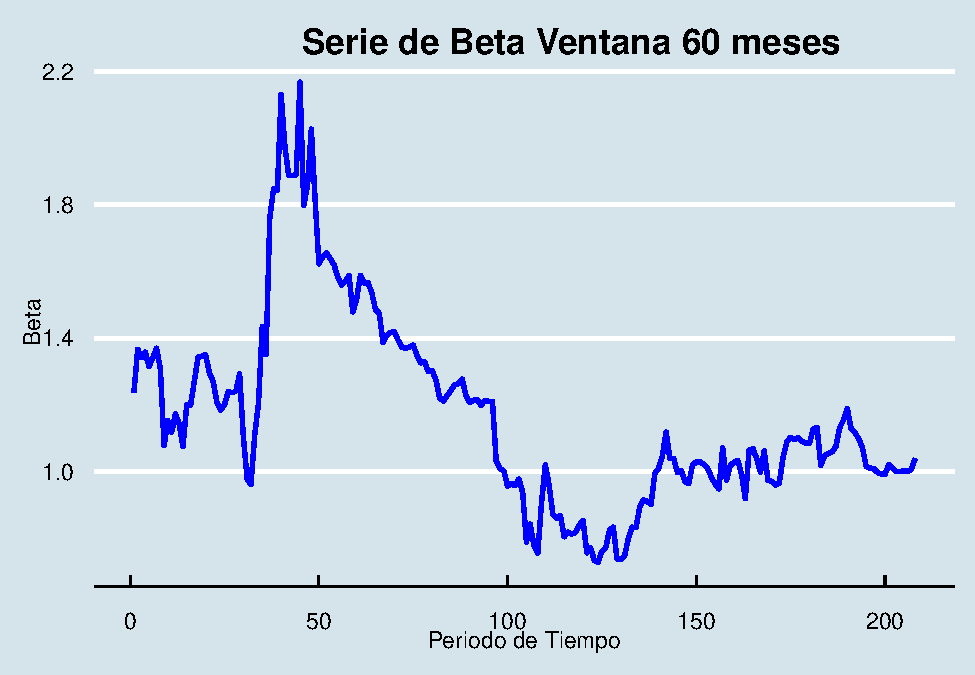
\includegraphics[width=0.95\linewidth]{figurasR/unnamed-chunk-16-1} \end{center}

Tal como podemos apreciar en el grafico anterior, la beta de Apple no es
constante en el tiempo y tienen una serie de variaciones hasta tal punto
de empezarse a estabilizarse en el tiempo, claramente una beta mayor a
1.0 nos da indicios de que es un activo más riesgoso que el mercado,
muchas veces dicho riesgo esta asociado a los proyectos que tiene la
compañía y las expectativas sobre si va o no ser rentable, sabemos que
Apple históricamente en sus inicios no era considerada una empresa cuyos
proyectos eran realizables, es por eso que alcanzó a presentar una beta
cercana a 2.2 con respecto al mercado, pero luego con el paso del
tiempo, logró mostrar que en verdad si lo era, a tal punto de que su
riesgo (Beta) fluctuara con respecto al mercado.

\hypertarget{performance-of-colombian-pension-funds.}{%
\section{Performance of Colombian Pension
Funds.}\label{performance-of-colombian-pension-funds.}}

Descargue una serie mensual de 10 años de rendimientos para cada una de
las cuatro compañías administradoras de fondos de pensiones obligatorias
en Colombia (use el ``Portafolio Moderado'').

\begin{Shaded}
\begin{Highlighting}[]
\NormalTok{Fondos }\OtherTok{\textless{}{-}} \FunctionTok{read\_excel}\NormalTok{(}\StringTok{"retornos\_fondos.xlsx"}\NormalTok{)}
\FunctionTok{head}\NormalTok{(Fondos)}
\end{Highlighting}
\end{Shaded}

\begin{verbatim}
## # A tibble: 6 x 7
##   DATE                PROTECCION PORVENIR  SKANDIA COLFONDOS `MSCI -DTF`
##   <dttm>                   <dbl>    <dbl>    <dbl>     <dbl>       <dbl>
## 1 2011-02-01 00:00:00    0.00426  0.00816  0.00322   0.00412     0.0525 
## 2 2011-03-01 00:00:00   -0.132   -0.0430  -0.124    -0.121      -0.0340 
## 3 2011-04-01 00:00:00    0.00390  0.00939  0.00719   0.00669    -0.0353 
## 4 2011-05-01 00:00:00    0.0206   0.0209   0.0162    0.0216      0.00642
## 5 2011-06-01 00:00:00   -0.0102  -0.00817 -0.00505  -0.0102     -0.0389 
## 6 2011-07-01 00:00:00   -0.00150 -0.00284 -0.00897  -0.00296    -0.0492 
## # ... with 1 more variable: `COLCAP - DTF` <dbl>
\end{verbatim}

\begin{Shaded}
\begin{Highlighting}[]
\NormalTok{RG }\OtherTok{\textless{}{-}}\NormalTok{ Fondos}\SpecialCharTok{$}\StringTok{\textasciigrave{}}\AttributeTok{MSCI {-}DTF}\StringTok{\textasciigrave{}}
\NormalTok{RL }\OtherTok{\textless{}{-}}\NormalTok{ Fondos}\SpecialCharTok{$}\StringTok{\textasciigrave{}}\AttributeTok{COLCAP {-} DTF}\StringTok{\textasciigrave{}}
\NormalTok{Xfondos }\OtherTok{\textless{}{-}} \FunctionTok{cbind}\NormalTok{(}\DecValTok{1}\NormalTok{,RG,RL)}
\NormalTok{PROTECCION }\OtherTok{\textless{}{-}} \FunctionTok{cbind}\NormalTok{(Fondos}\SpecialCharTok{$}\NormalTok{PROTECCION)}
\NormalTok{PORVENIR}\OtherTok{\textless{}{-}} \FunctionTok{cbind}\NormalTok{(Fondos}\SpecialCharTok{$}\NormalTok{PORVENIR)}
\NormalTok{SKANDIA}\OtherTok{\textless{}{-}} \FunctionTok{cbind}\NormalTok{(Fondos}\SpecialCharTok{$}\NormalTok{SKANDIA)}
\NormalTok{COLFONDOS}\OtherTok{\textless{}{-}} \FunctionTok{cbind}\NormalTok{(Fondos}\SpecialCharTok{$}\NormalTok{COLFONDOS)}
\end{Highlighting}
\end{Shaded}

\hypertarget{estimaciuxf3n-de-capm-mix}{%
\subsection{Estimación de CAPM Mix}\label{estimaciuxf3n-de-capm-mix}}

Vamos a estimar un CAPM `mixto' donde la cartera de mercado incluye
tanto los rendimientos de un índice de renta variable internacional (los
rendimientos de una cartera de renta variable global en COP sobre el
activo libre de riesgo, RG) como el rendimiento del mercado de renta
variable nacional (rendimiento del COLCAP sobre el activo libre de
riesgo, RL). Para cada fondo de pensiones, hay que estimar la siguiente
ecuación: \[
R_{it}=\alpha_i+\beta_i\bullet{RG}_t+\gamma_i\bullet{RL}_t+\varepsilon_{it}
\]

Para la estimación del CAPM mixto, vamos a utilizar los rendimientos de
el MSCI index Global, el cual esta compuesto por las empresas más
rentables en los diferentes países desarrollados.

\begin{figure}
\centering
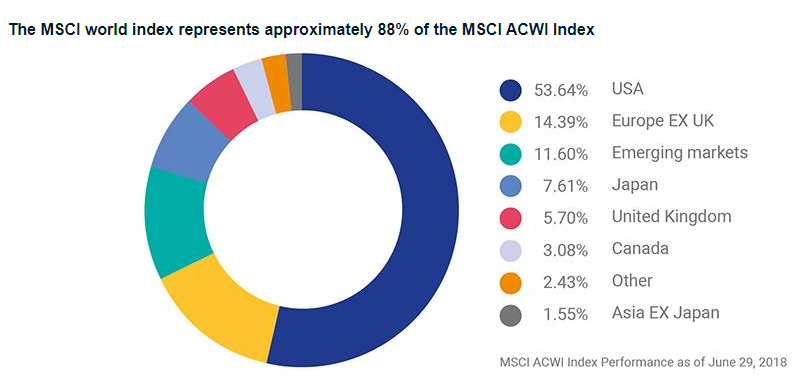
\includegraphics{index.png}
\caption{\textbf{MSCI INDEX}}
\end{figure}

Por otro lado, utilizamos el DTF como la tasa libre de riesgo y el
COLCAP como el índice de capital nacional.

\begin{itemize}
\item
  \textbf{VARIABLES}:

  -\emph{RG:} MSCI - DF

  -\emph{RL:} COLCAP -DF
\end{itemize}

Explicar cuál es el papel de los coeficientes, y qué nos dicen los
valores estimados sobre cada fondo de pensiones y su perfil de riesgo.
¿Son muy diferentes los coeficientes estimados? Explicar.

Creamos una

\begin{Shaded}
\begin{Highlighting}[]
\NormalTok{Beta\_function }\OtherTok{\textless{}{-}} \ControlFlowTok{function}\NormalTok{(X,Y)\{}
  \FunctionTok{solve}\NormalTok{(}\FunctionTok{t}\NormalTok{(X)}\SpecialCharTok{\%*\%}\NormalTok{X)}\SpecialCharTok{\%*\%}\FunctionTok{t}\NormalTok{(X)}\SpecialCharTok{\%*\%}\NormalTok{Y}
\NormalTok{\} }
\end{Highlighting}
\end{Shaded}

\begin{itemize}
\tightlist
\item
  \textbf{Fondo Proteccion:}
\end{itemize}

\begin{Shaded}
\begin{Highlighting}[]
\FunctionTok{Beta\_function}\NormalTok{(Xfondos,PROTECCION)}
\end{Highlighting}
\end{Shaded}

\begin{verbatim}
##           [,1]
##    0.007756745
## RG 0.280977765
## RL 0.080752784
\end{verbatim}

Para el fondo de proteccion podemos notar que el coeficiente que más
afecta el modelo es el RG, es decir el indice global, en comparación con
el coeficiente asociado a la varaible RL (cOLCAP).

\begin{itemize}
\tightlist
\item
  \textbf{Fondo Porvenir:}
\end{itemize}

\begin{Shaded}
\begin{Highlighting}[]
\FunctionTok{Beta\_function}\NormalTok{(Xfondos,PORVENIR)}
\end{Highlighting}
\end{Shaded}

\begin{verbatim}
##          [,1]
##    0.01052644
## RG 0.12648560
## RL 0.01466640
\end{verbatim}

Por otro lado, el portafolio moderado de pensiones de poervenir muestra
un mayor coeficiente en la variable RG.

\begin{itemize}
\tightlist
\item
  \textbf{Fondo Skandia:}
\end{itemize}

\begin{Shaded}
\begin{Highlighting}[]
\FunctionTok{Beta\_function}\NormalTok{(Xfondos,SKANDIA)}
\end{Highlighting}
\end{Shaded}

\begin{verbatim}
##           [,1]
##    0.006261861
## RG 0.145670188
## RL 0.016065416
\end{verbatim}

Así mismo para el caso del fondo Skandia el factor internacional
representado en el MSCI index Global, tiene un mayor impacto a
comparación con el Colcap.

\begin{itemize}
\tightlist
\item
  \textbf{Fondo Colfondos:}
\end{itemize}

\begin{Shaded}
\begin{Highlighting}[]
\FunctionTok{Beta\_function}\NormalTok{(Xfondos,COLFONDOS)}
\end{Highlighting}
\end{Shaded}

\begin{verbatim}
##          [,1]
##    0.00459223
## RG 0.17499049
## RL 0.02442653
\end{verbatim}

Finalmente para el caso del fondo COLFONDOS, este tambien tiene un
coeficiente alto para la variable RG, en comparación con el RL

\hypertarget{macro-factor-model}{%
\subsection{Macro-factor model:}\label{macro-factor-model}}

\begin{Shaded}
\begin{Highlighting}[]
\NormalTok{macro\_factors }\OtherTok{\textless{}{-}} \FunctionTok{read\_excel}\NormalTok{(}\StringTok{"macro\_factors.xlsx"}\NormalTok{)}
\end{Highlighting}
\end{Shaded}

\begin{Shaded}
\begin{Highlighting}[]
\NormalTok{TRM }\OtherTok{\textless{}{-}} \FunctionTok{cbind}\NormalTok{(macro\_factors}\SpecialCharTok{$}\NormalTok{TRM)}
\NormalTok{TES }\OtherTok{\textless{}{-}} \FunctionTok{cbind}\NormalTok{(macro\_factors}\SpecialCharTok{$}\NormalTok{TES)}
\NormalTok{IPC }\OtherTok{\textless{}{-}} \FunctionTok{cbind}\NormalTok{(macro\_factors}\SpecialCharTok{$}\NormalTok{IPC)}
\NormalTok{Xfondos1 }\OtherTok{\textless{}{-}} \FunctionTok{cbind}\NormalTok{(}\DecValTok{1}\NormalTok{,RG,RL,TRM,TES,IPC)}
\FunctionTok{colnames}\NormalTok{(Xfondos1)}\OtherTok{\textless{}{-}}\FunctionTok{c}\NormalTok{(}\StringTok{"Intercepto"}\NormalTok{,}\StringTok{"RG"}\NormalTok{,}\StringTok{"RL"}\NormalTok{,}\StringTok{"TRM"}\NormalTok{,}\StringTok{"TES"}\NormalTok{,}\StringTok{"IPC"}\NormalTok{)}
\end{Highlighting}
\end{Shaded}

Para poder continuar con nuestro análisis que nos permita explicar de
dónde provienen los rendimientos de los fondos de pensiones colombianos,
ahora a nuestro modelo empleado anteriormente, vamos agregarle 3
factores más, pero en este caso serán factores macroeconómicos tales
como la tasa de referencia del mercado (TRM), la tasa de los TES a 1 año
y finalmente el IPC, pues consideramos que estas variables pueden darnos
más indicios para llegar a una conclusión final acerca de las
rentabilidades de los fondos de inversión, para eso utilizaremos la
siguiente ecuación.

\[
R_{it}=\alpha_i+\beta_i\bullet{RG}_t+\gamma_i\bullet{RL}_t+b_1F_1+b_2F_2+b_3F_3+\varepsilon_{it}
\]

Para iniciar corremos la regresión para los diferentes fondos de
pensiones y posteriormente realizamos un análisis sobre las variables de
cada uno.

\begin{itemize}
\tightlist
\item
  \textbf{Fondo Proteccion:}
\end{itemize}

\begin{Shaded}
\begin{Highlighting}[]
\FunctionTok{Beta\_function}\NormalTok{(Xfondos1,PROTECCION)}
\end{Highlighting}
\end{Shaded}

\begin{verbatim}
##                    [,1]
## Intercepto  0.002607842
## RG          0.429827757
## RL          0.089779546
## TRM        -0.351218129
## TES         0.128348703
## IPC        -0.027073114
\end{verbatim}

Para el fondo protección podemos notar que hay un cambio en los
coeficientes con respecto a la anterior regresión del mismo fondo
podemos notar que el intercepto es casi cero por lo que las
rentabilidades dadas por el fondo son acertadas, Por otro lado el
coeficiente que más significancia tienen el modelo es del factor
internacional, pues es de 0.4298, Así mismo el factor macroeconómico de
test tiene también una alta significancia en el modelo 0.1283 y
finalmente variables como la TRM y el IPC Son coeficientes que afectan
al modelo de forma negativa.

\begin{itemize}
\tightlist
\item
  \textbf{Fondo Porvenir:}
\end{itemize}

\begin{Shaded}
\begin{Highlighting}[]
\FunctionTok{Beta\_function}\NormalTok{(Xfondos1,PORVENIR)}
\end{Highlighting}
\end{Shaded}

\begin{verbatim}
##                     [,1]
## Intercepto  0.0082956663
## RG          0.1842382867
## RL          0.0172084432
## TRM        -0.1377165975
## TES         0.0003877277
## IPC         0.8169784463
\end{verbatim}

Continuando con el análisis y teniendo factores macroeconómicos podemos
ver que en el caso de porvenir los coeficientes del IPC e
internacionales como el MSCI index Global, son altos por lo que podemos
concluir que las rentabilidades de las pensiones obligatorias del fondo
porvenir están más ligadas a las expectativas de inflación que presenta
el país, como también a un factor internacional, sin embargo el
coeficiente de los TEST es casi cero por lo que podríamos afirmar que no
tiene una relación con los títulos de renta fija nacionales, sin embargo
no significa que su portafolio no tenga está clase de títulos pues
podrían ser internacionales.

\begin{itemize}
\tightlist
\item
  \textbf{Fondo Skandia:}
\end{itemize}

\begin{Shaded}
\begin{Highlighting}[]
\FunctionTok{Beta\_function}\NormalTok{(Xfondos1,SKANDIA)}
\end{Highlighting}
\end{Shaded}

\begin{verbatim}
##                    [,1]
## Intercepto -0.006966852
## RG          0.265387673
## RL          0.023806050
## TRM        -0.257713967
## TES         0.296938161
## IPC        -0.100874568
\end{verbatim}

Por otro lado el fondo de pensiones skandia a diferencia del fondo
porvenir los coeficientes de IPC como el de la TRM son negativos, En
este caso el intercepto es negativo por lo que podríamos inferir que las
rentabilidades generadas estarían por debajo de las esperadas por parte
de los inversionistas, en la misma línea de análisis los dos factores
con mayor significancia son los del mercado de renta variable
internacional y los de TES colombianos.

\begin{itemize}
\tightlist
\item
  \textbf{Fondo Colfondos:}
\end{itemize}

\begin{Shaded}
\begin{Highlighting}[]
\FunctionTok{Beta\_function}\NormalTok{(Xfondos1,COLFONDOS)}
\end{Highlighting}
\end{Shaded}

\begin{verbatim}
##                    [,1]
## Intercepto -0.001394781
## RG          0.292469914
## RL          0.031825175
## TRM        -0.271587364
## TES         0.151944491
## IPC        -0.185308611
\end{verbatim}

Finalmente haciendo un análisis al fondo de pensiones Colfondos, podemos
notar que la variable internacional y los TEST colombianos tienen el
mayor coeficiente, esto nos podría dar indicios que las rentabilidades
de dicho fondo están más sujetas a los mercados internacionales que
locales debido a que el factor RL (COLCAP) es significativamente
pequeño, también podemos destacar que los factores como la TRM y IPC son
significativamente negativos.

  \bibliography{bib/library.bib,bib/paquetes.bib}

\end{document}
